\section{Runtime View}

In this section, the most relevant sequence diagrams are shown to describe the way components interact to accomplish specific tasks of the application.

\subsection{Customer Login}
This sequence diagram shows the login procedure executed by a Customer. \\
Firstly, after having opened the CLup MobileApplication on his smartphone, an already registered Customer fills in the form with his username and password. Then a first simple check is actuated by the MobileApplication itself, which controls whether one or both these two fields are missing, and in that case it shows an error message. Conversely, if this is not the case, the AccountManager is contacted and this component, in turn, propagates the request to the DatabaseAccess that provides the access to the Database, where all the users credentials are stored permanently. Therefore, if in the Database there is couple of values username and password that matches the one inserted by the Customer, then the login is successfully completed, otherwise an error message is shown. \\
Notice that, even if not represented in these sequence diagrams, an analogous procedure, based on the WebApplication and AuthenticationService components, can obviously be done also by the Store Manager.
\begin{figure}[H]
\centerline{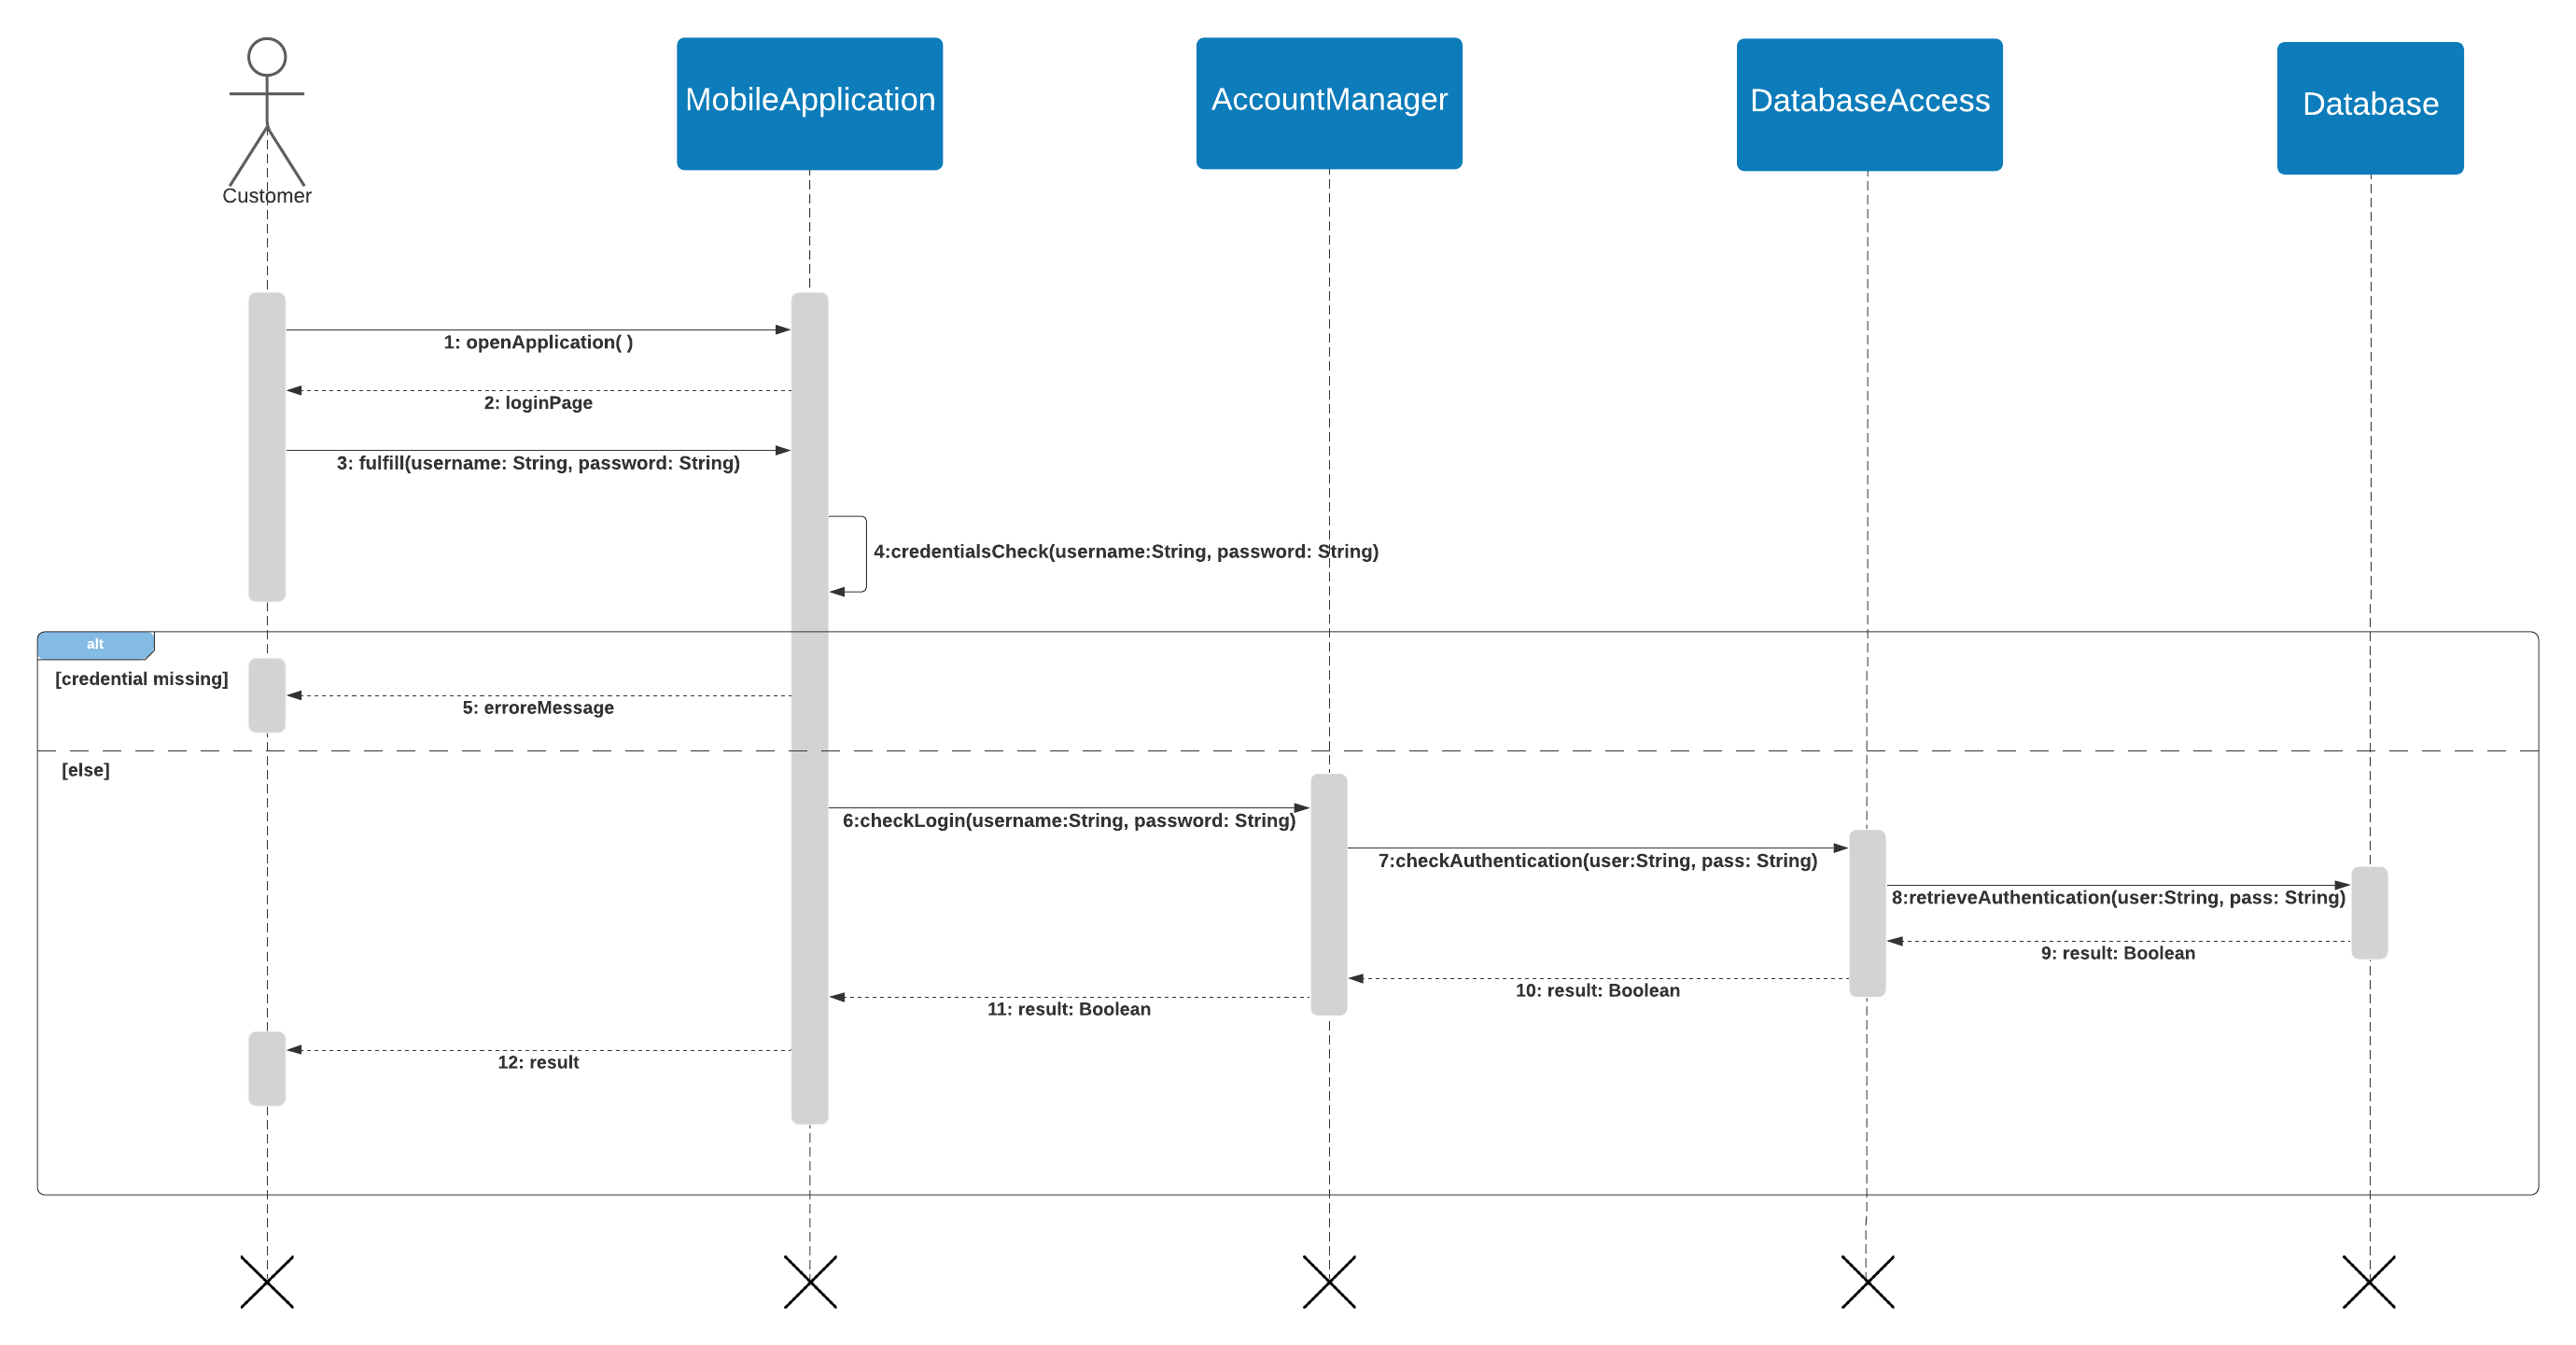
\includegraphics[scale=0.45]{./CustomerLoginSequenceDD}}
\caption{Customer Login Sequence Diagram}
\end{figure}

\subsection{Store Manager Registration}
In this sequence diagram it is shown the process of registration attended by the Store Manager. The Store Manager, using his own computer, after having switched from the login page to the registration one, does the registration filling in the form with his personal username, email, password and the certificate file. Then, the WebApplication controls that all the credentials and the certificate are indicated and that the passwords do not mismatch. Then, the registration request is sent from the WebApplication to the AuthenticationService component. After, this last one calls the DatabaseAccess component to store the information in the Database. So, the result of this operation is propagated back to the Store Manager, following in reverse order the same path as before, and if the result is positive the registration is successful, otherwise it should be repeated.
\begin{figure}[H]
\centerline{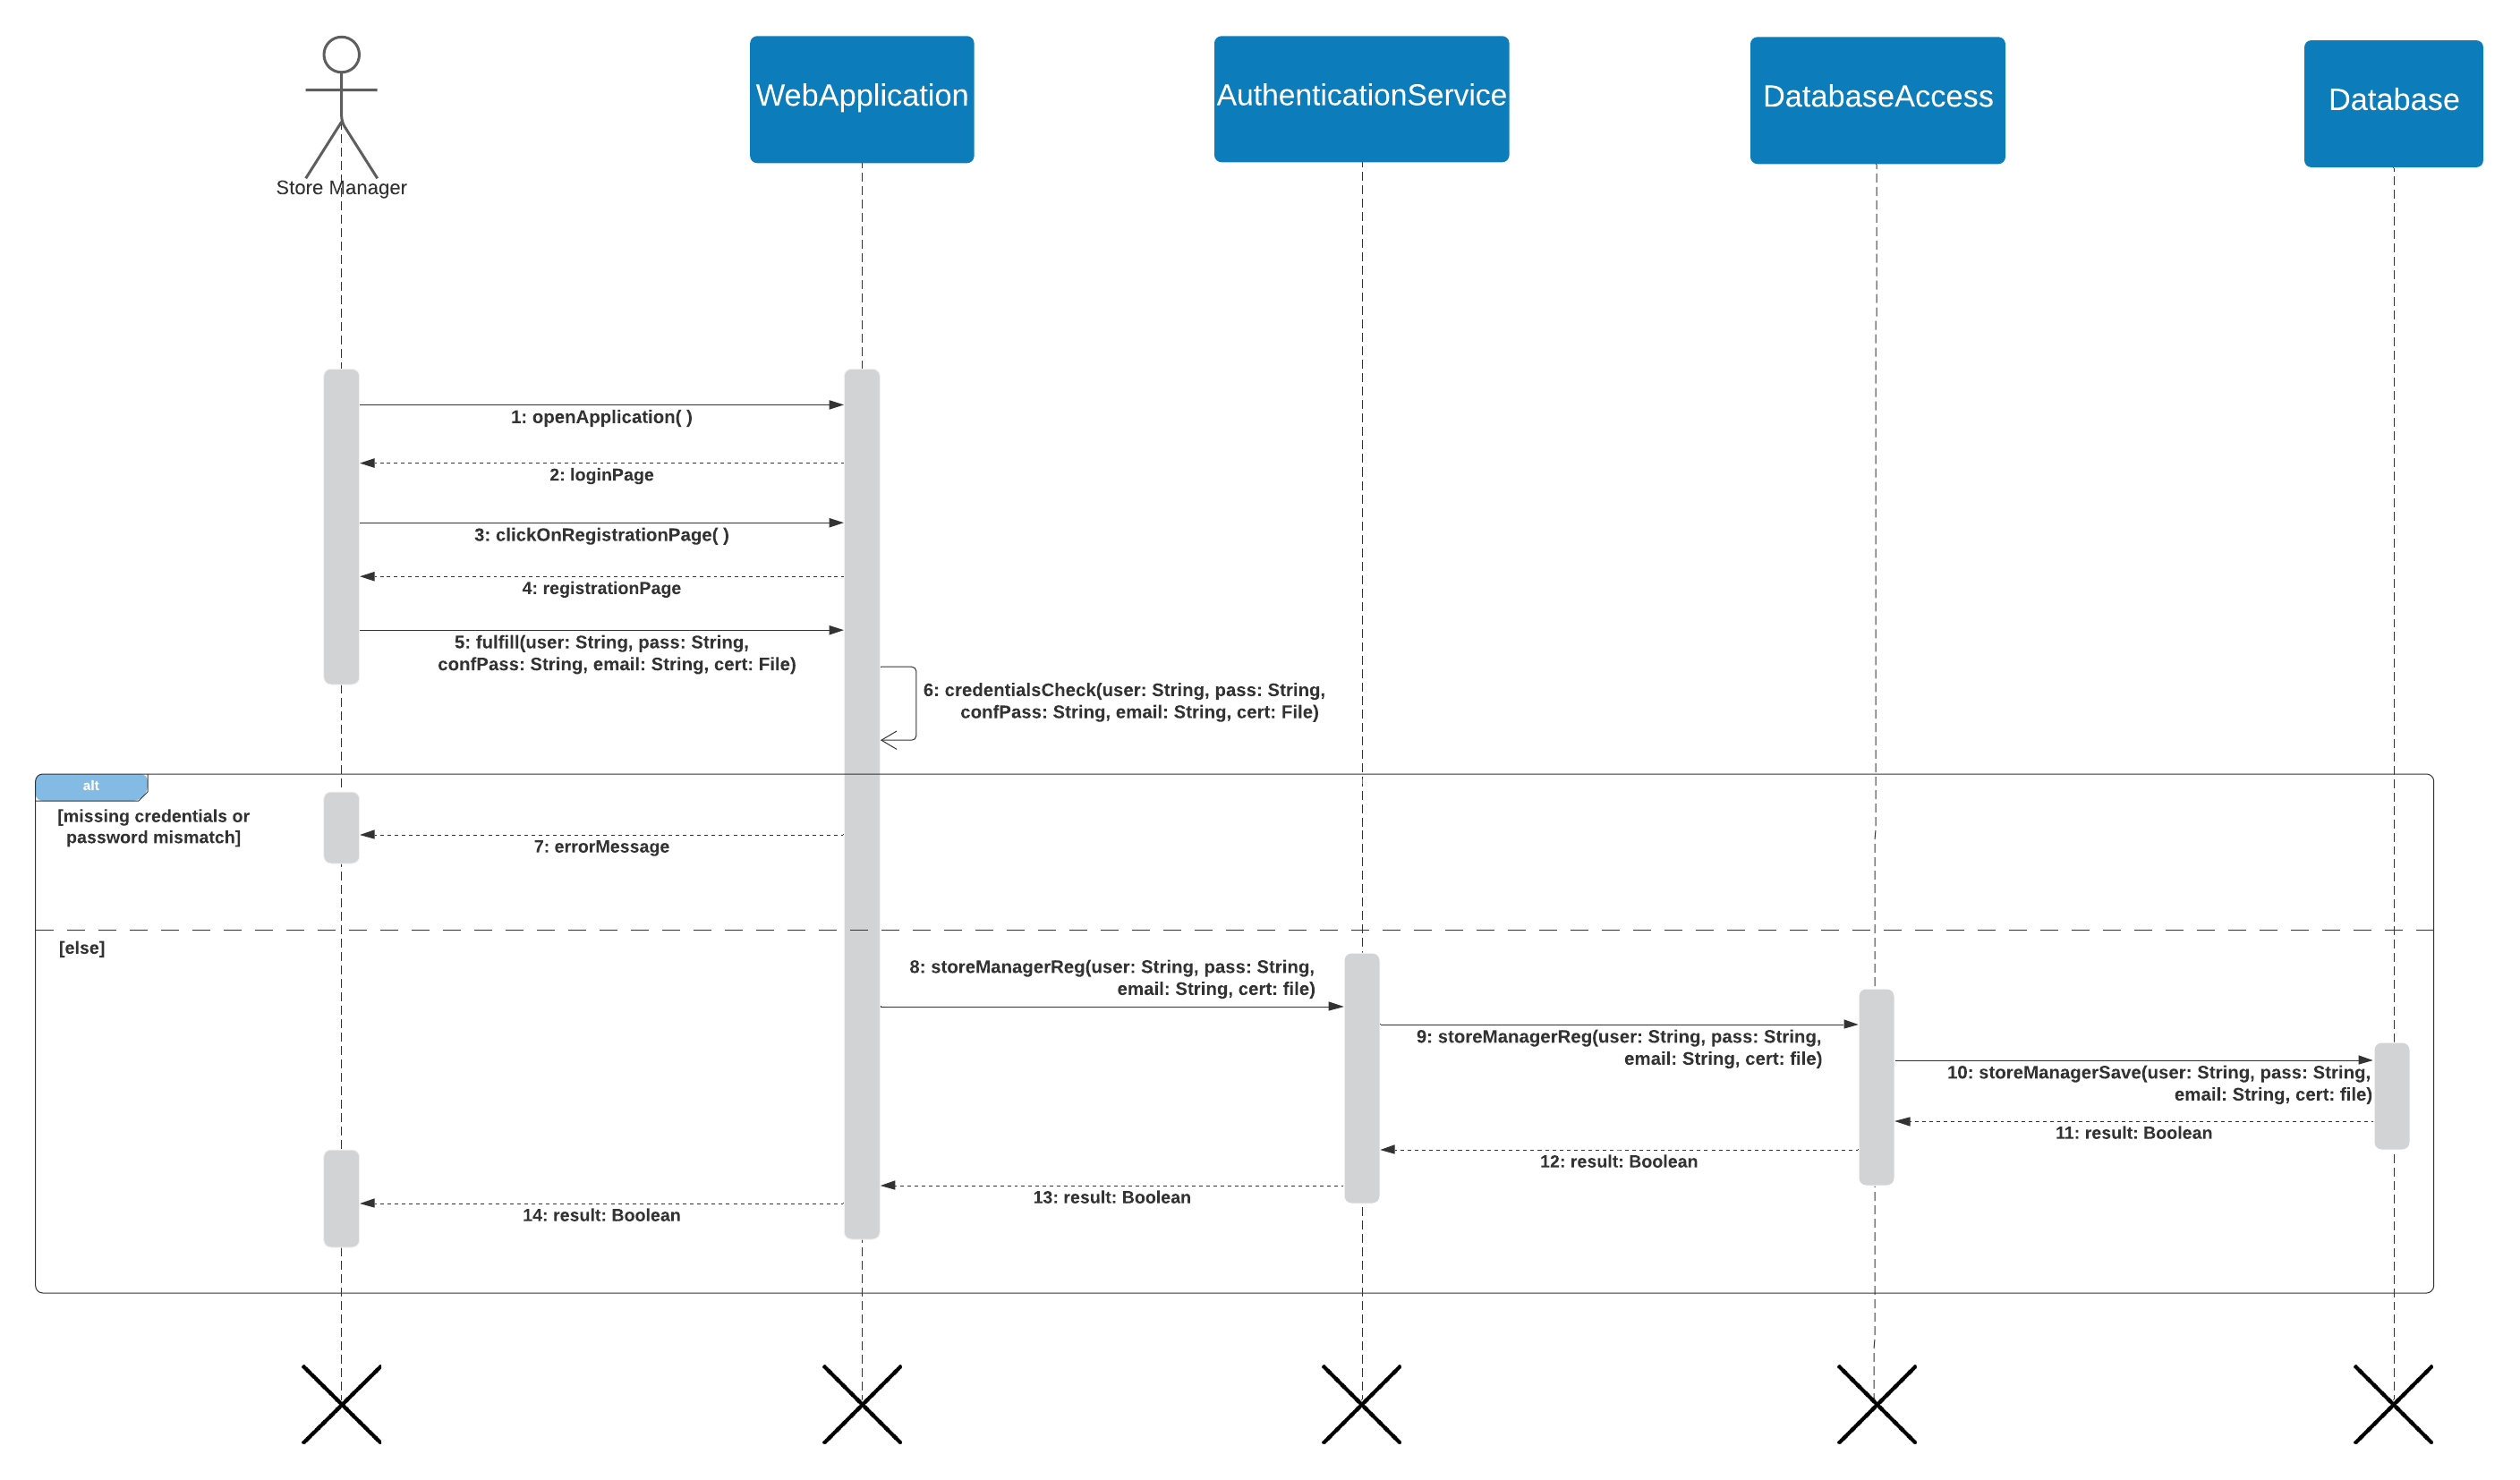
\includegraphics[scale=0.45]{./StoreManagerRegistrationSequenceDD}}
\caption{Store Manager Registration Sequence Diagram}
\end{figure}

\subsection{Line-Up Request}
This sequence diagram is used to show the Line-Up process. \\
Firstly, after having clicked on the Line-Up tab, the Customer selects the supermarket and the means of transport he intends to use to reach the store. The MobileApplication checks if all the data have been inserted and are correct, then it sends the LineUpRequest to the LineUpService component in the Application Server. The LineUpService, in turn, calls the RealTimeQueueManager to add the Customer to the Real-Time Queue and to compute his Waiting Time; then, it generates the corrispondent QR Code and returns the LineUpRequest to the MobileApplication, so that the Customer is shown all the useful informations. \\
Notice that the the RealTimeQueueManager does not have to access every time the Database, because it is updated periodically.
\begin{figure}[H]
\centerline{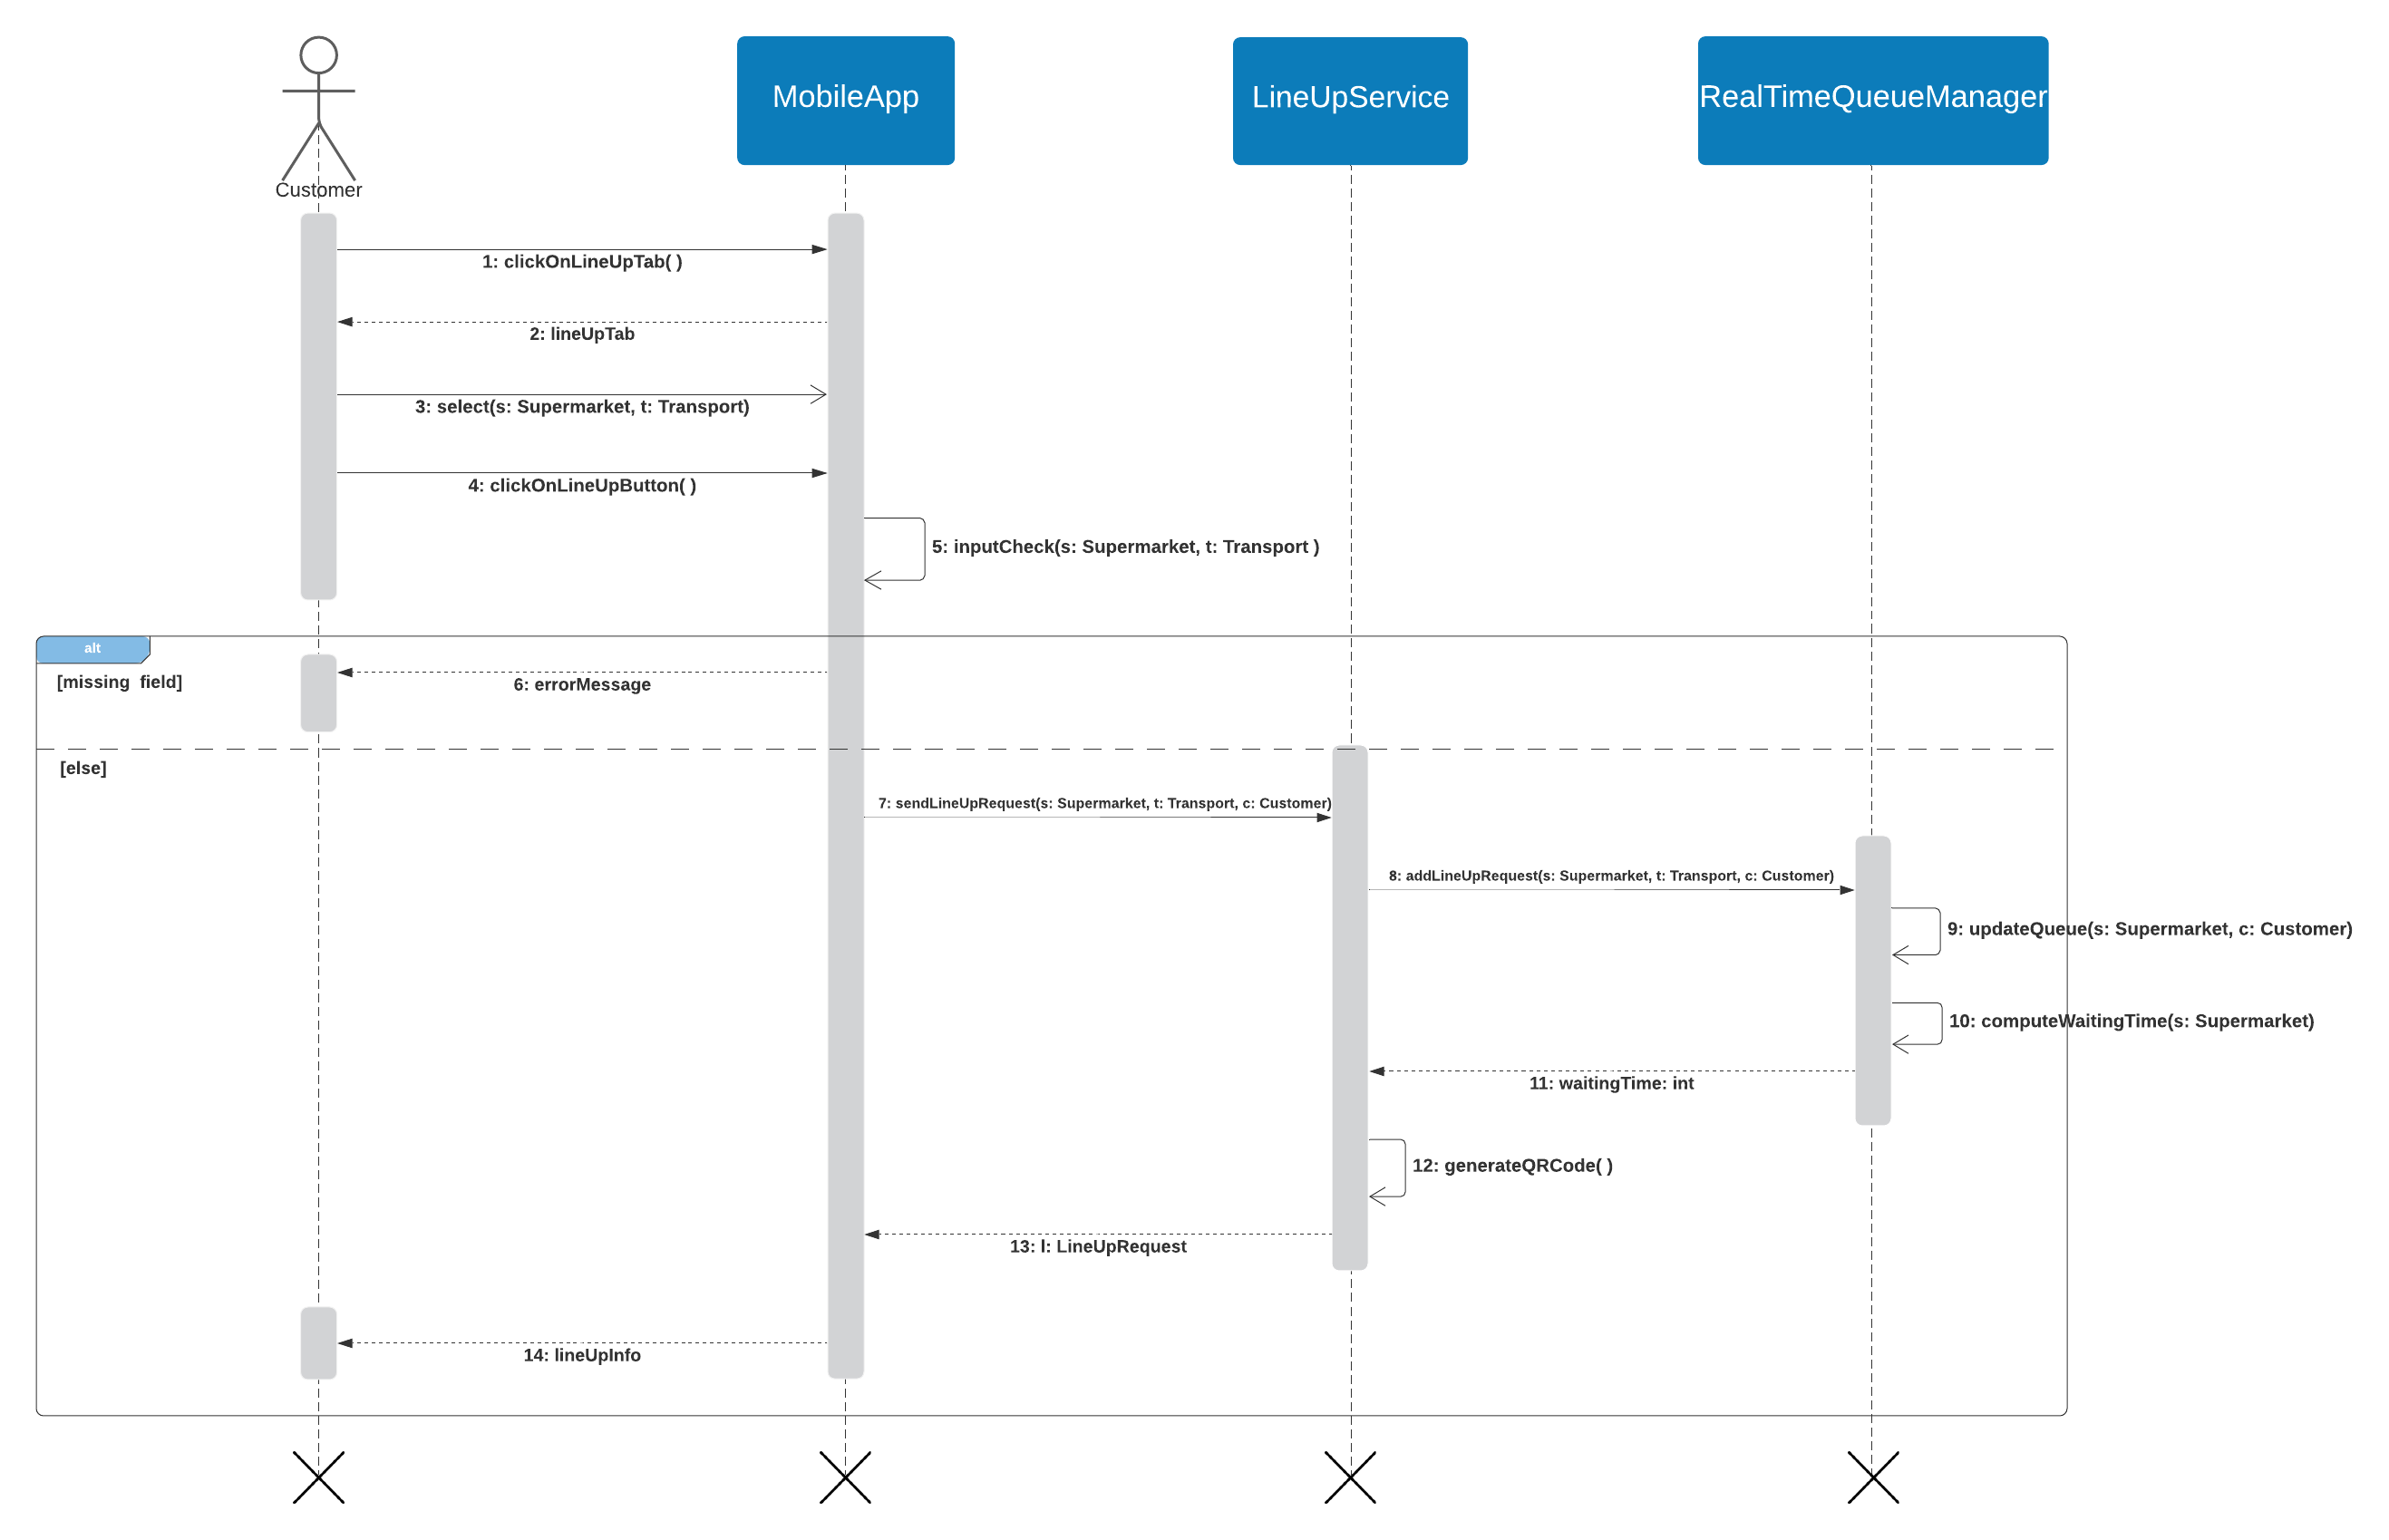
\includegraphics[scale=0.5]{./LineUpSequenceDD}}
\caption{Line-Up Sequence Diagram}
\end{figure}


\subsection{Booking Request}
This sequence diagram is used to show the Booking Process.\\
Firstly, after having clicked on the Booking tab, an already logged-in Customer selects the supermarket. The MobileApplication uses the BookingService, DatabaseAccess and Database components to retrieve the time slots where the supermarket is open and not full. Then, if the Customer is not a Long-Term one, he must necessary indicate the Expected Duration of his visit, while instead, if he is a Long-Term one, this information is not mandatory.
Moreover, both kinds of Customers can, optionally, indicate the list of items, or their categories, that they intend to buy. Once clicked the Book button, the MobileApplication checks if all the data have been inserted and are correct, then it sends the BookingRequest to the BookingService component in the Application Server. This last one infers the Expected Duration for those Long-Term Customers that have not indicated explicitly the ExpectedDuration, and, thanks to the DatabaseAccess and Database components, store the Booking in the Database. Finally, it update the AADs for the visit-optimizations (see section 2.8.2) and returns the Booking to the MobileApplication, so that the Customer is shown all the useful informations.
\begin{figure}[H]
\centerline{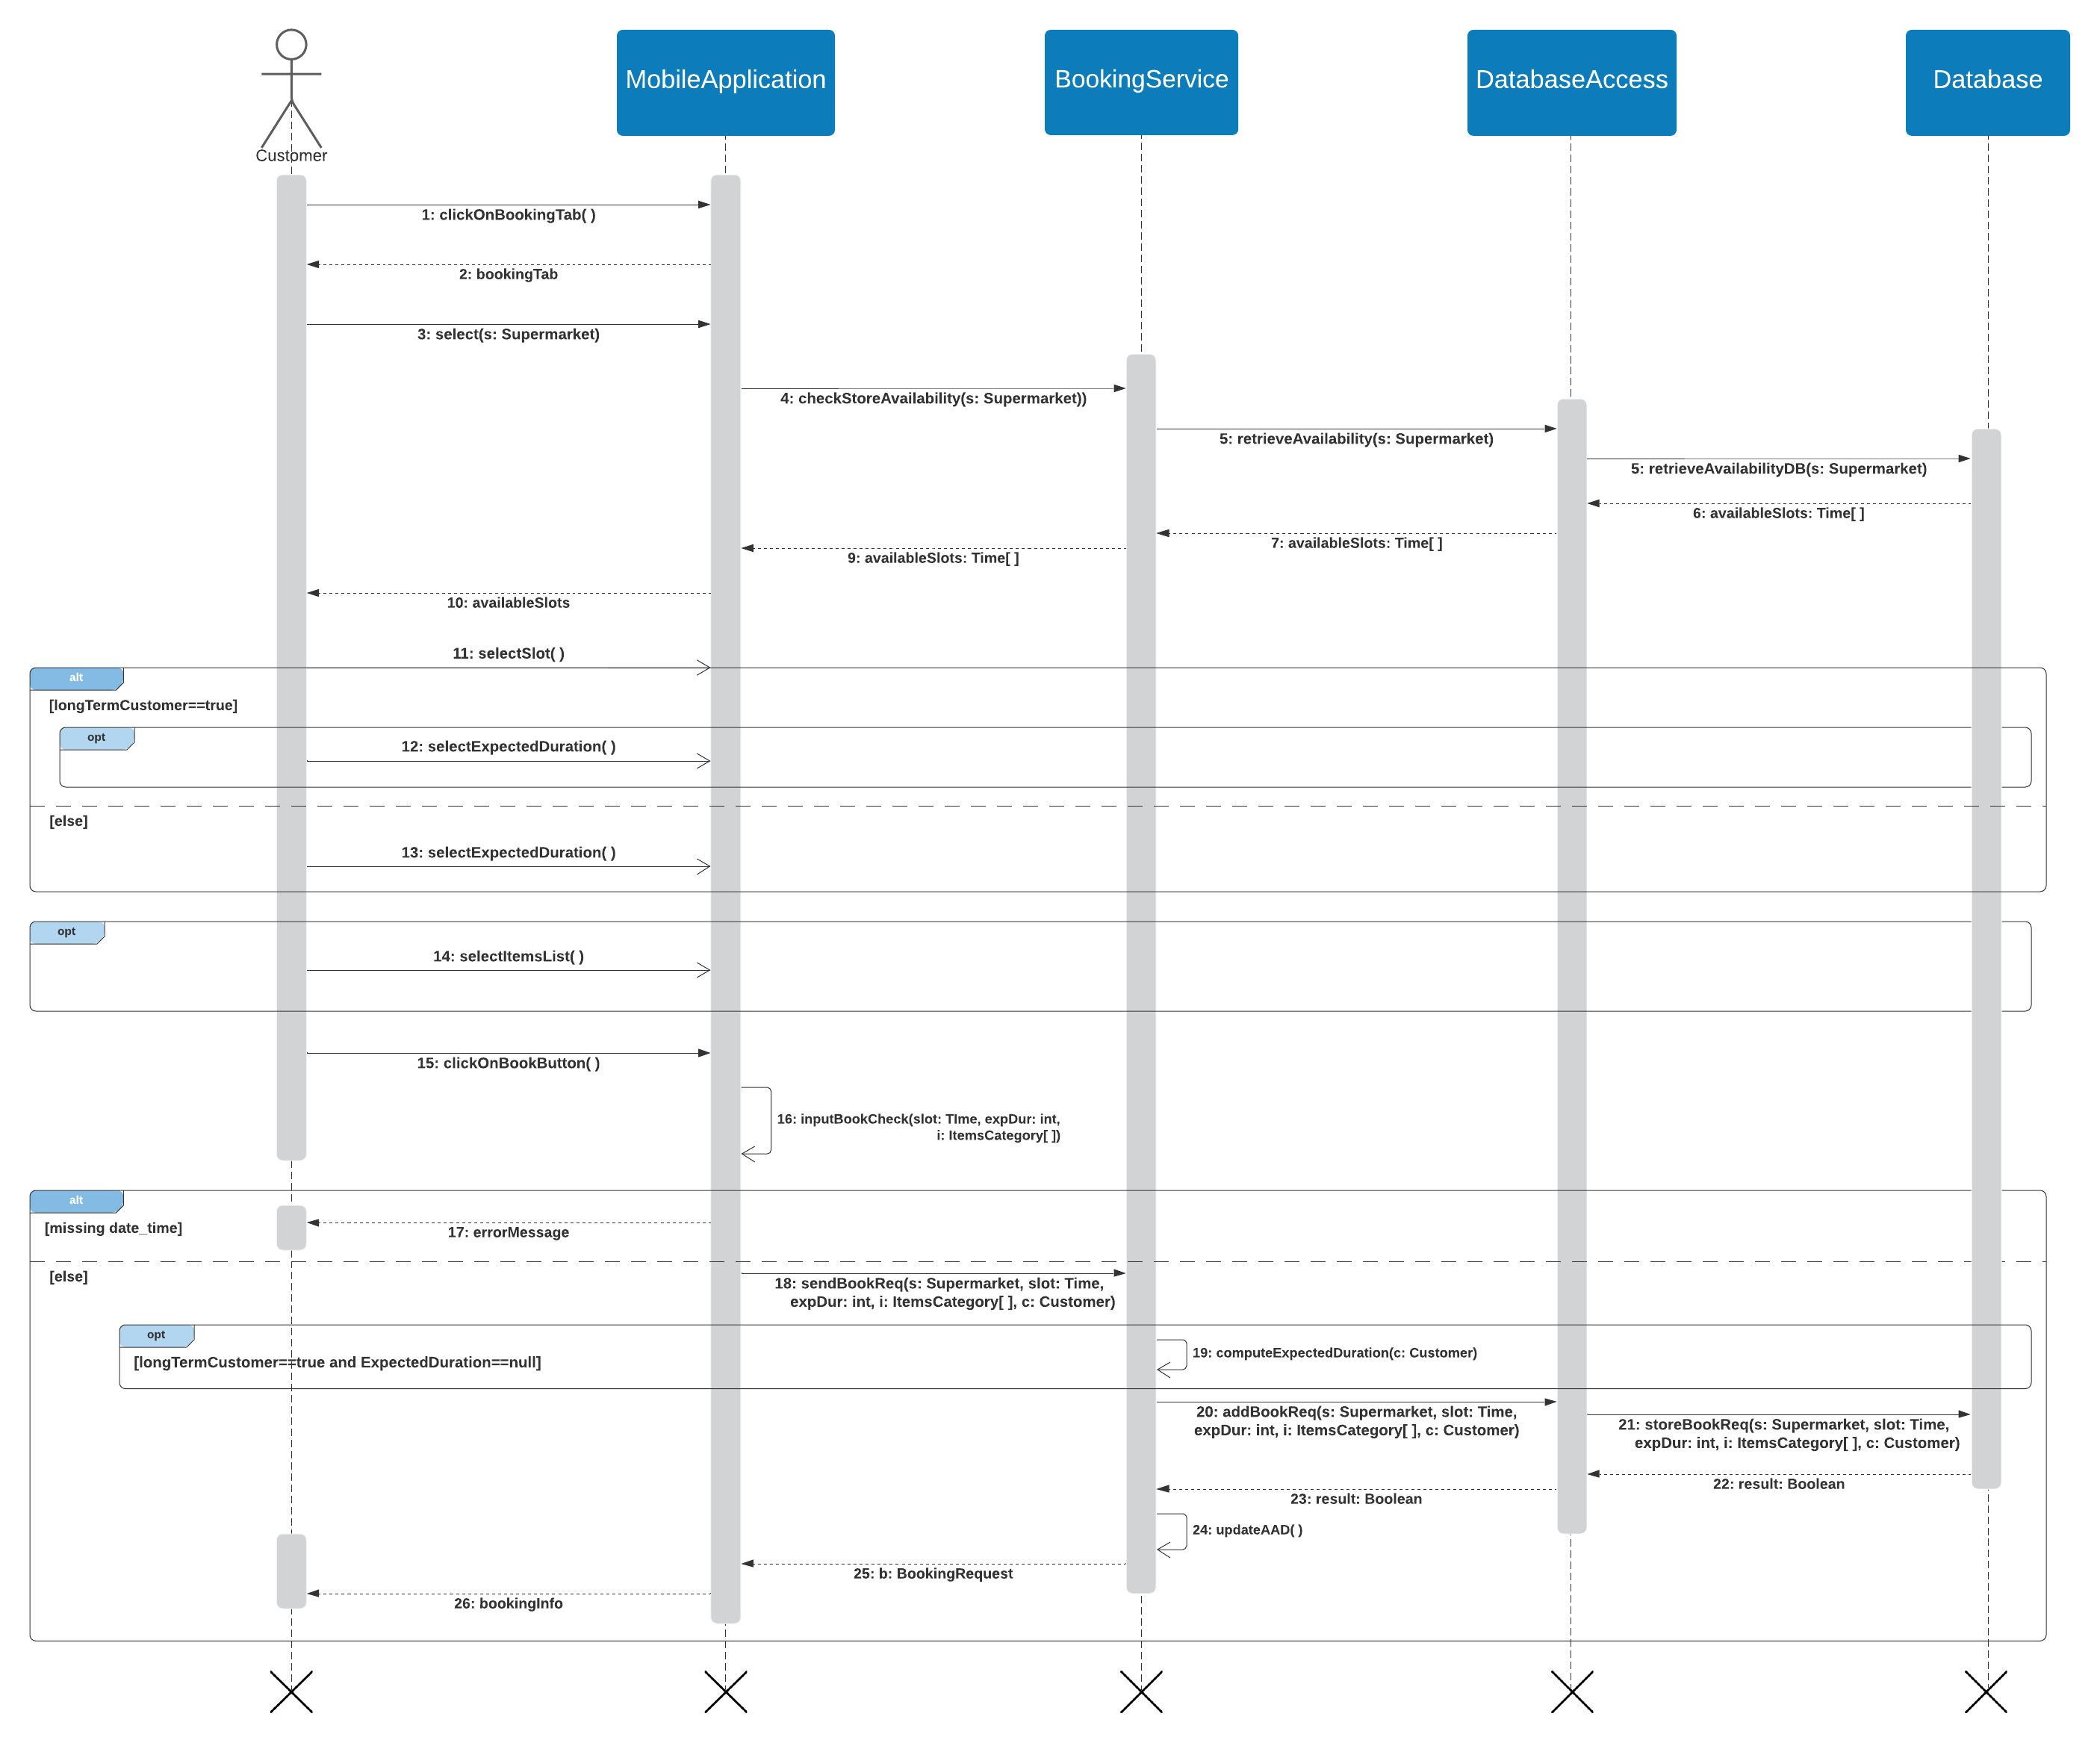
\includegraphics[scale=0.45]{./BookingSequenceDD}}
\caption{Booking Sequence Diagram}
\end{figure}


\subsection{Cancel Line-Up}
This sequence diagram shows the produre of cancelling a Line-Up performed by the an already lined-up Customer: if instead a Customer has not an active LineUpRequest, he cannot try to do this operation, since the cancel button is displayed only in this case, as presented and explained in the User Interface section. \\
Firstly, after having clicked on the LineUpTab and then on the the mentioned button, the request is propagated from the MobileApplication to the LineUpService. \\ Subsequently, the LineUpService forwards the request to the RealTimeQueueManager that deletes the LineUpRequest from the queue. Finally, a confirmation message is propagated back to the Customer. 
\begin{figure}[H]
\centerline{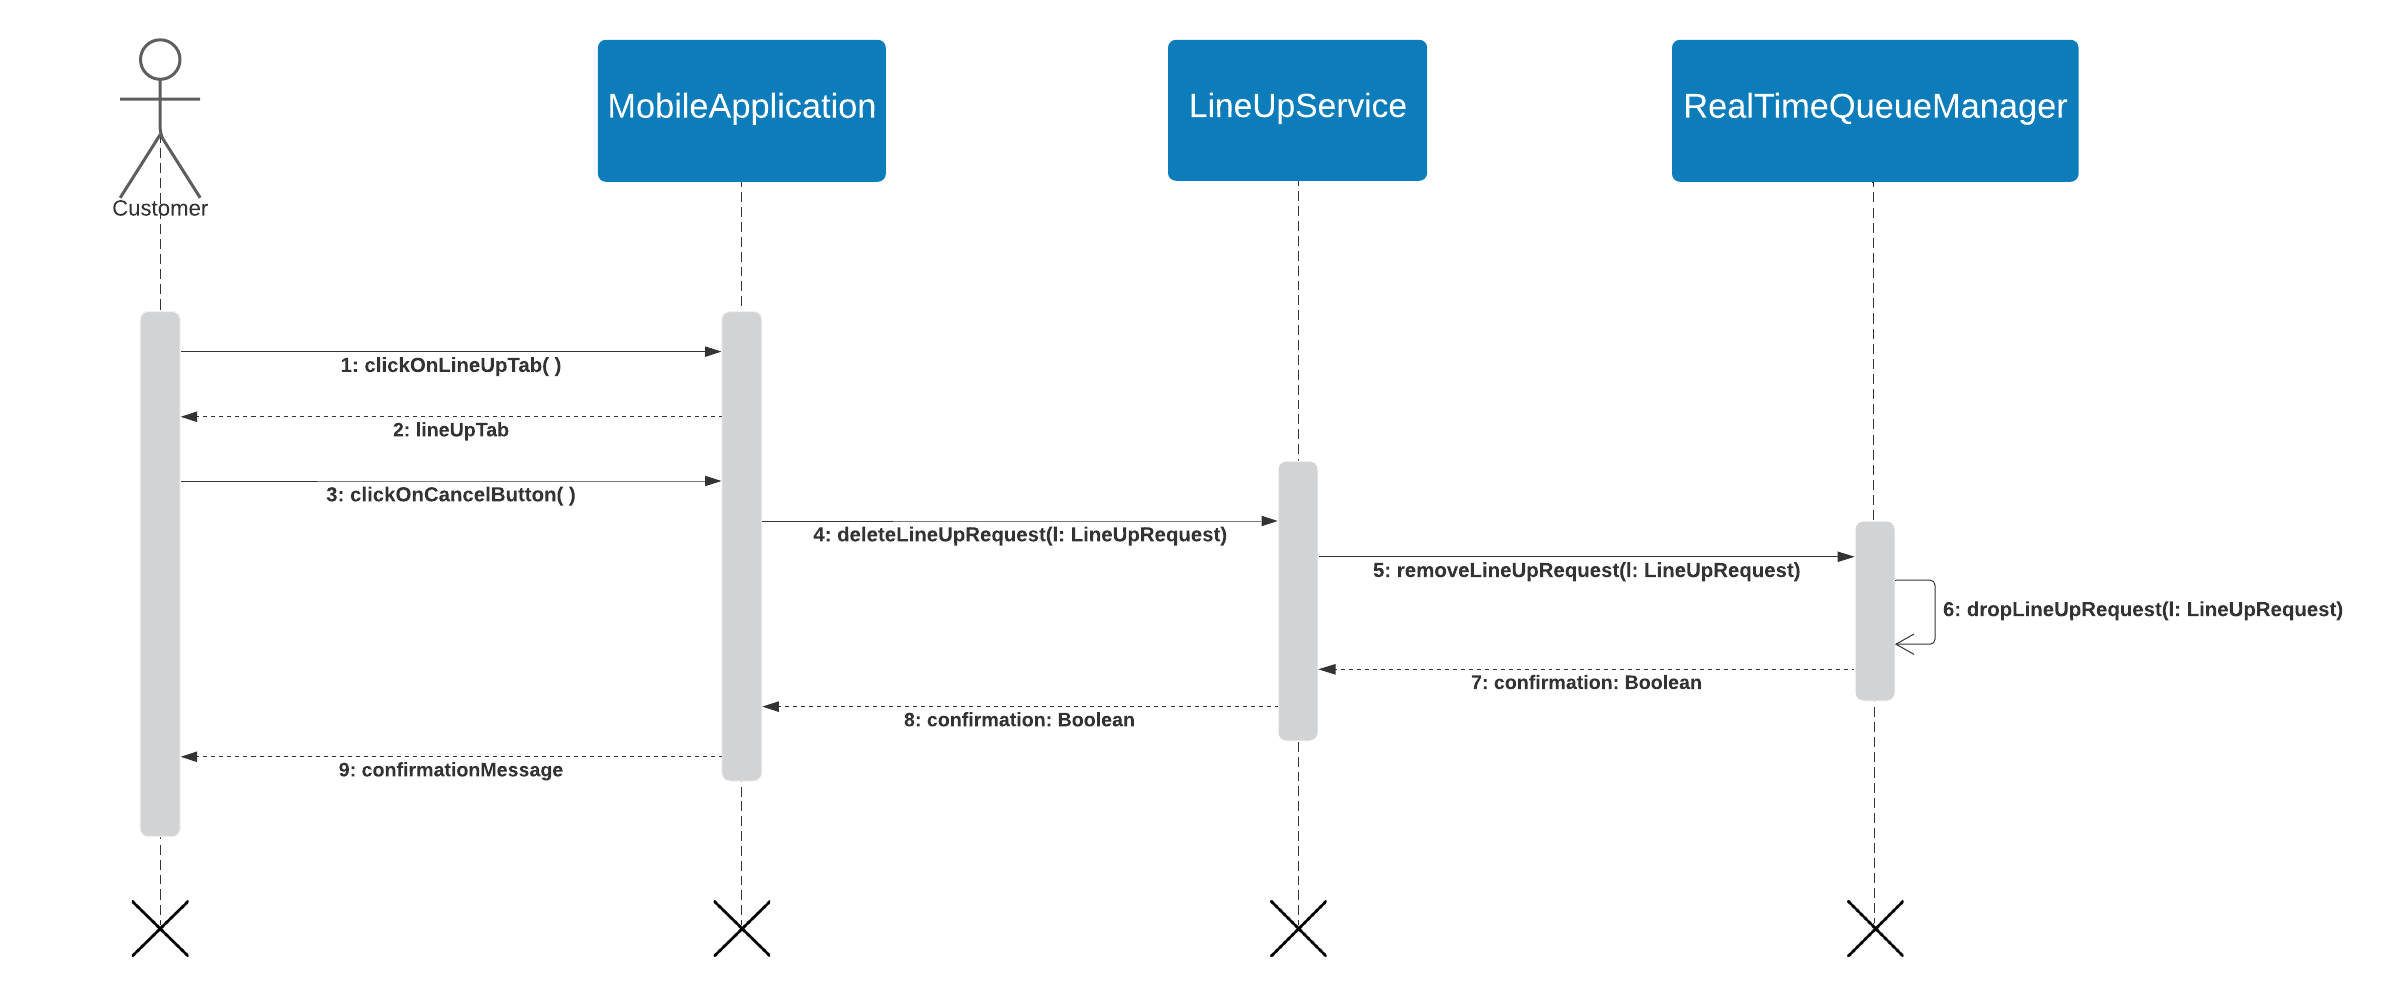
\includegraphics[scale=0.5]{./CancelLineUpSequenceDD}}
\caption{Cancel Line-Up Sequence Diagram}
\end{figure}


\subsection{Cancel Booking}
This sequence diagram shows the produre of cancelling a Booking performed by the an already booked Customer: if instead a Customer has not an active BookingRequest, he cannot try to do this operation, since the cancel button is displayed only in this case, as presented and explained in the User Interface section. \\
Firstly, after having clicked on the BookingTab and then on the the mentioned button, the request is propagated from the MobileApplication to the BookingService. \\ Subsequently, the BookingService forwards the request to the DatabaseAccess that provides the access to the Database from which the BookingRequest is deleted through an SQL query. Finally, a confirmation message is propagated back to the Customer. 		\\
Notice that if the Booking was already in the RealTimeQueueManager, it will be removed at the next periodical update.
\begin{figure}[H]
\centerline{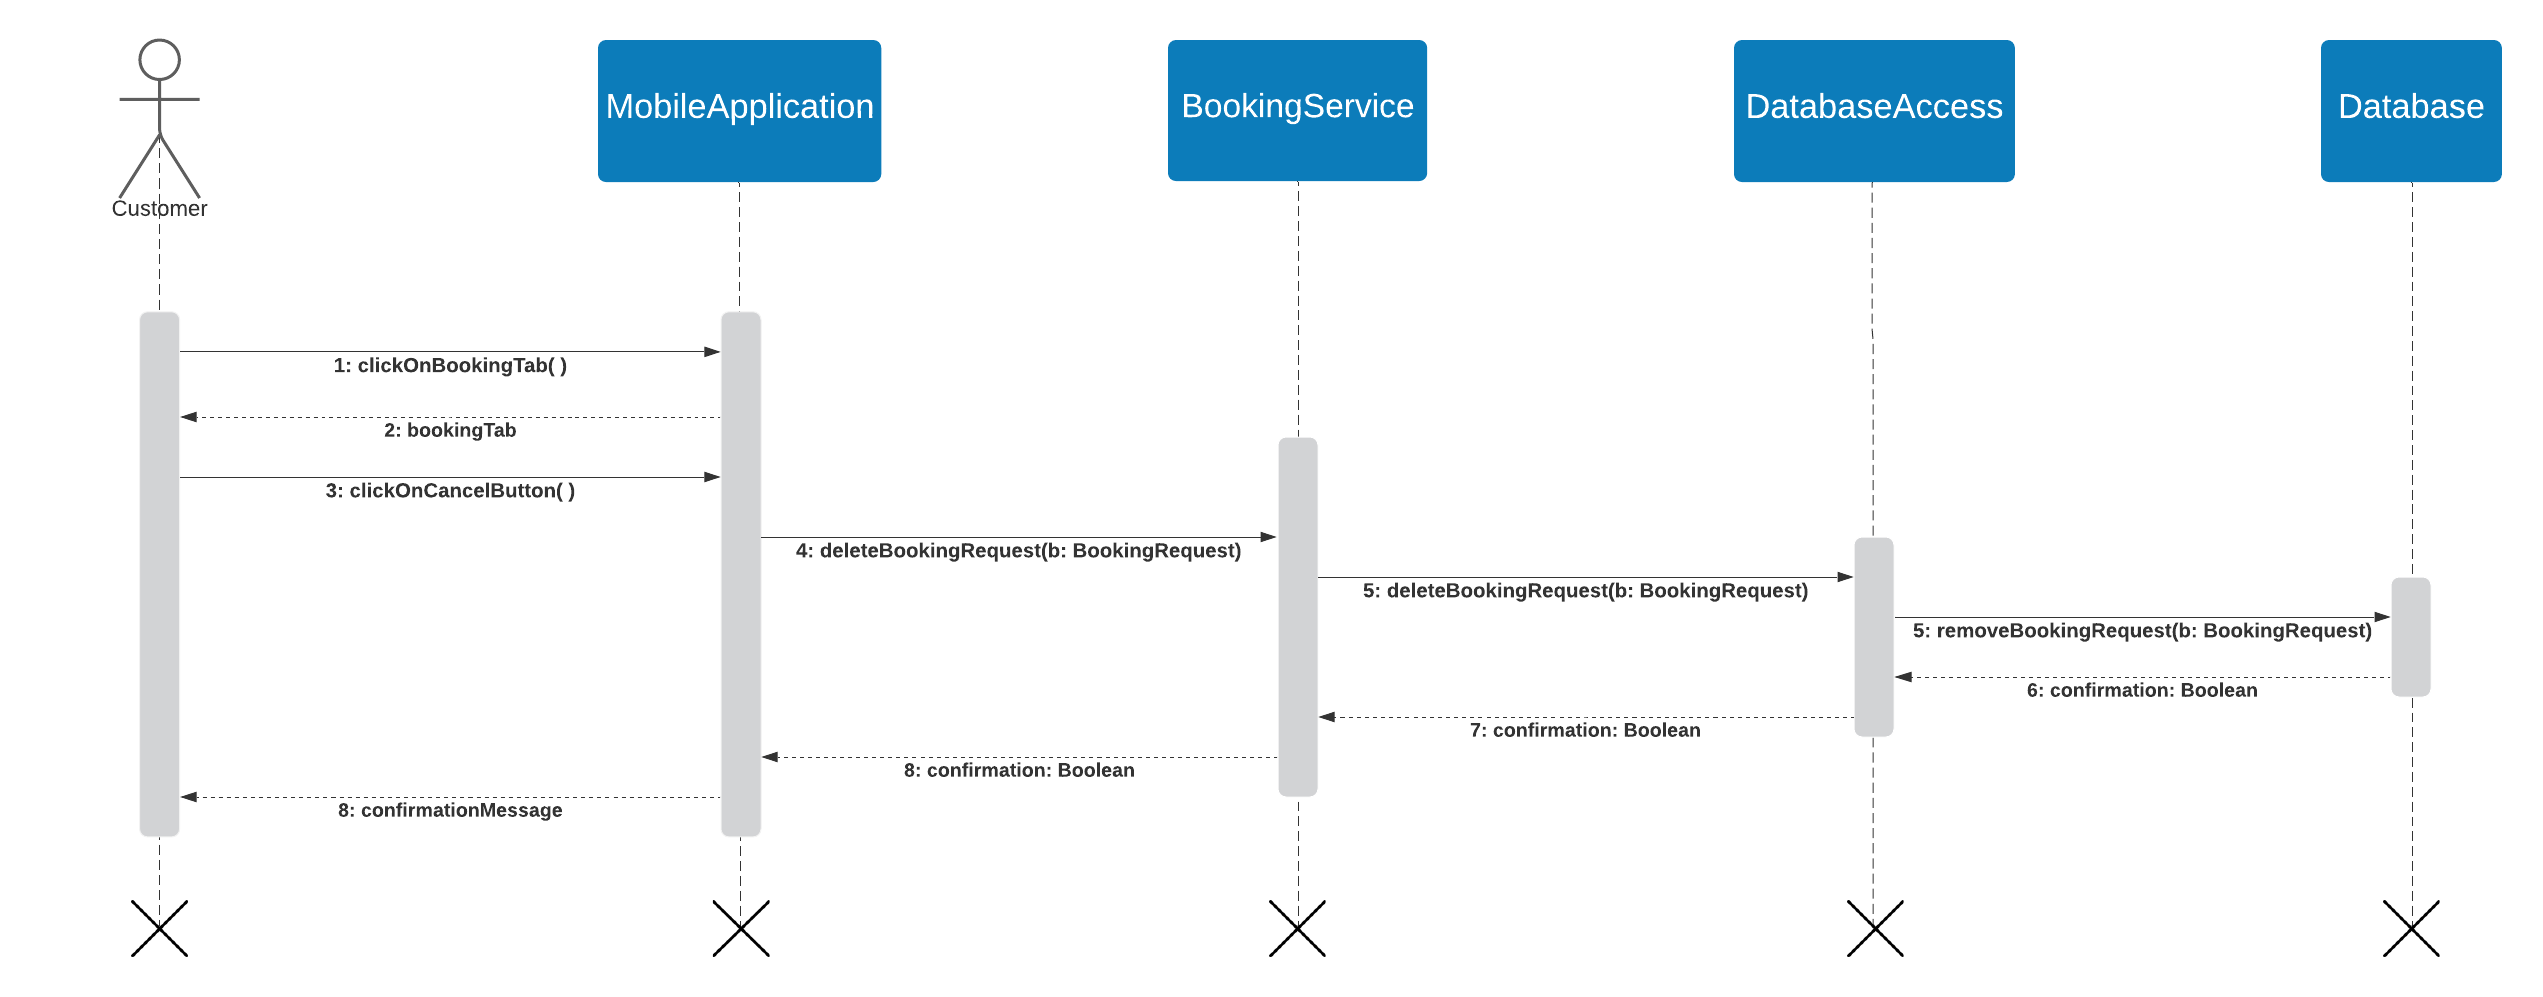
\includegraphics[scale=0.5]{./CancelBookingSequenceDD}}
\caption{Cancel Booking Sequence Diagram}
\end{figure}


\subsection{Ticket Generation}
This sequence diagram shows the procedure, performed by Store Managers, for generating a Ticket in case a Non-Tech Customer arrives at the supermarket.\\
Firstly, after having clicked on the NewTicket button, the WebApplication check whether the supermarket is full calling the TicketService, which ,in turn, retrieves this information from the RealTimeQueueManager. In fact, if the supermarket is full, the No-Tech Customer will have to wait that at least one Customer exits the store before entering, in order to always respect the maximum capiency. Therefore, if there is enough space the TicketService generates a new Ticket and the RealTimeQueueManager gets updated counting this new entrance. Otherwise, if the store is full, an error message is shown and the Store Manager will have to repeat the operation. 
\begin{figure}[H]
\centerline{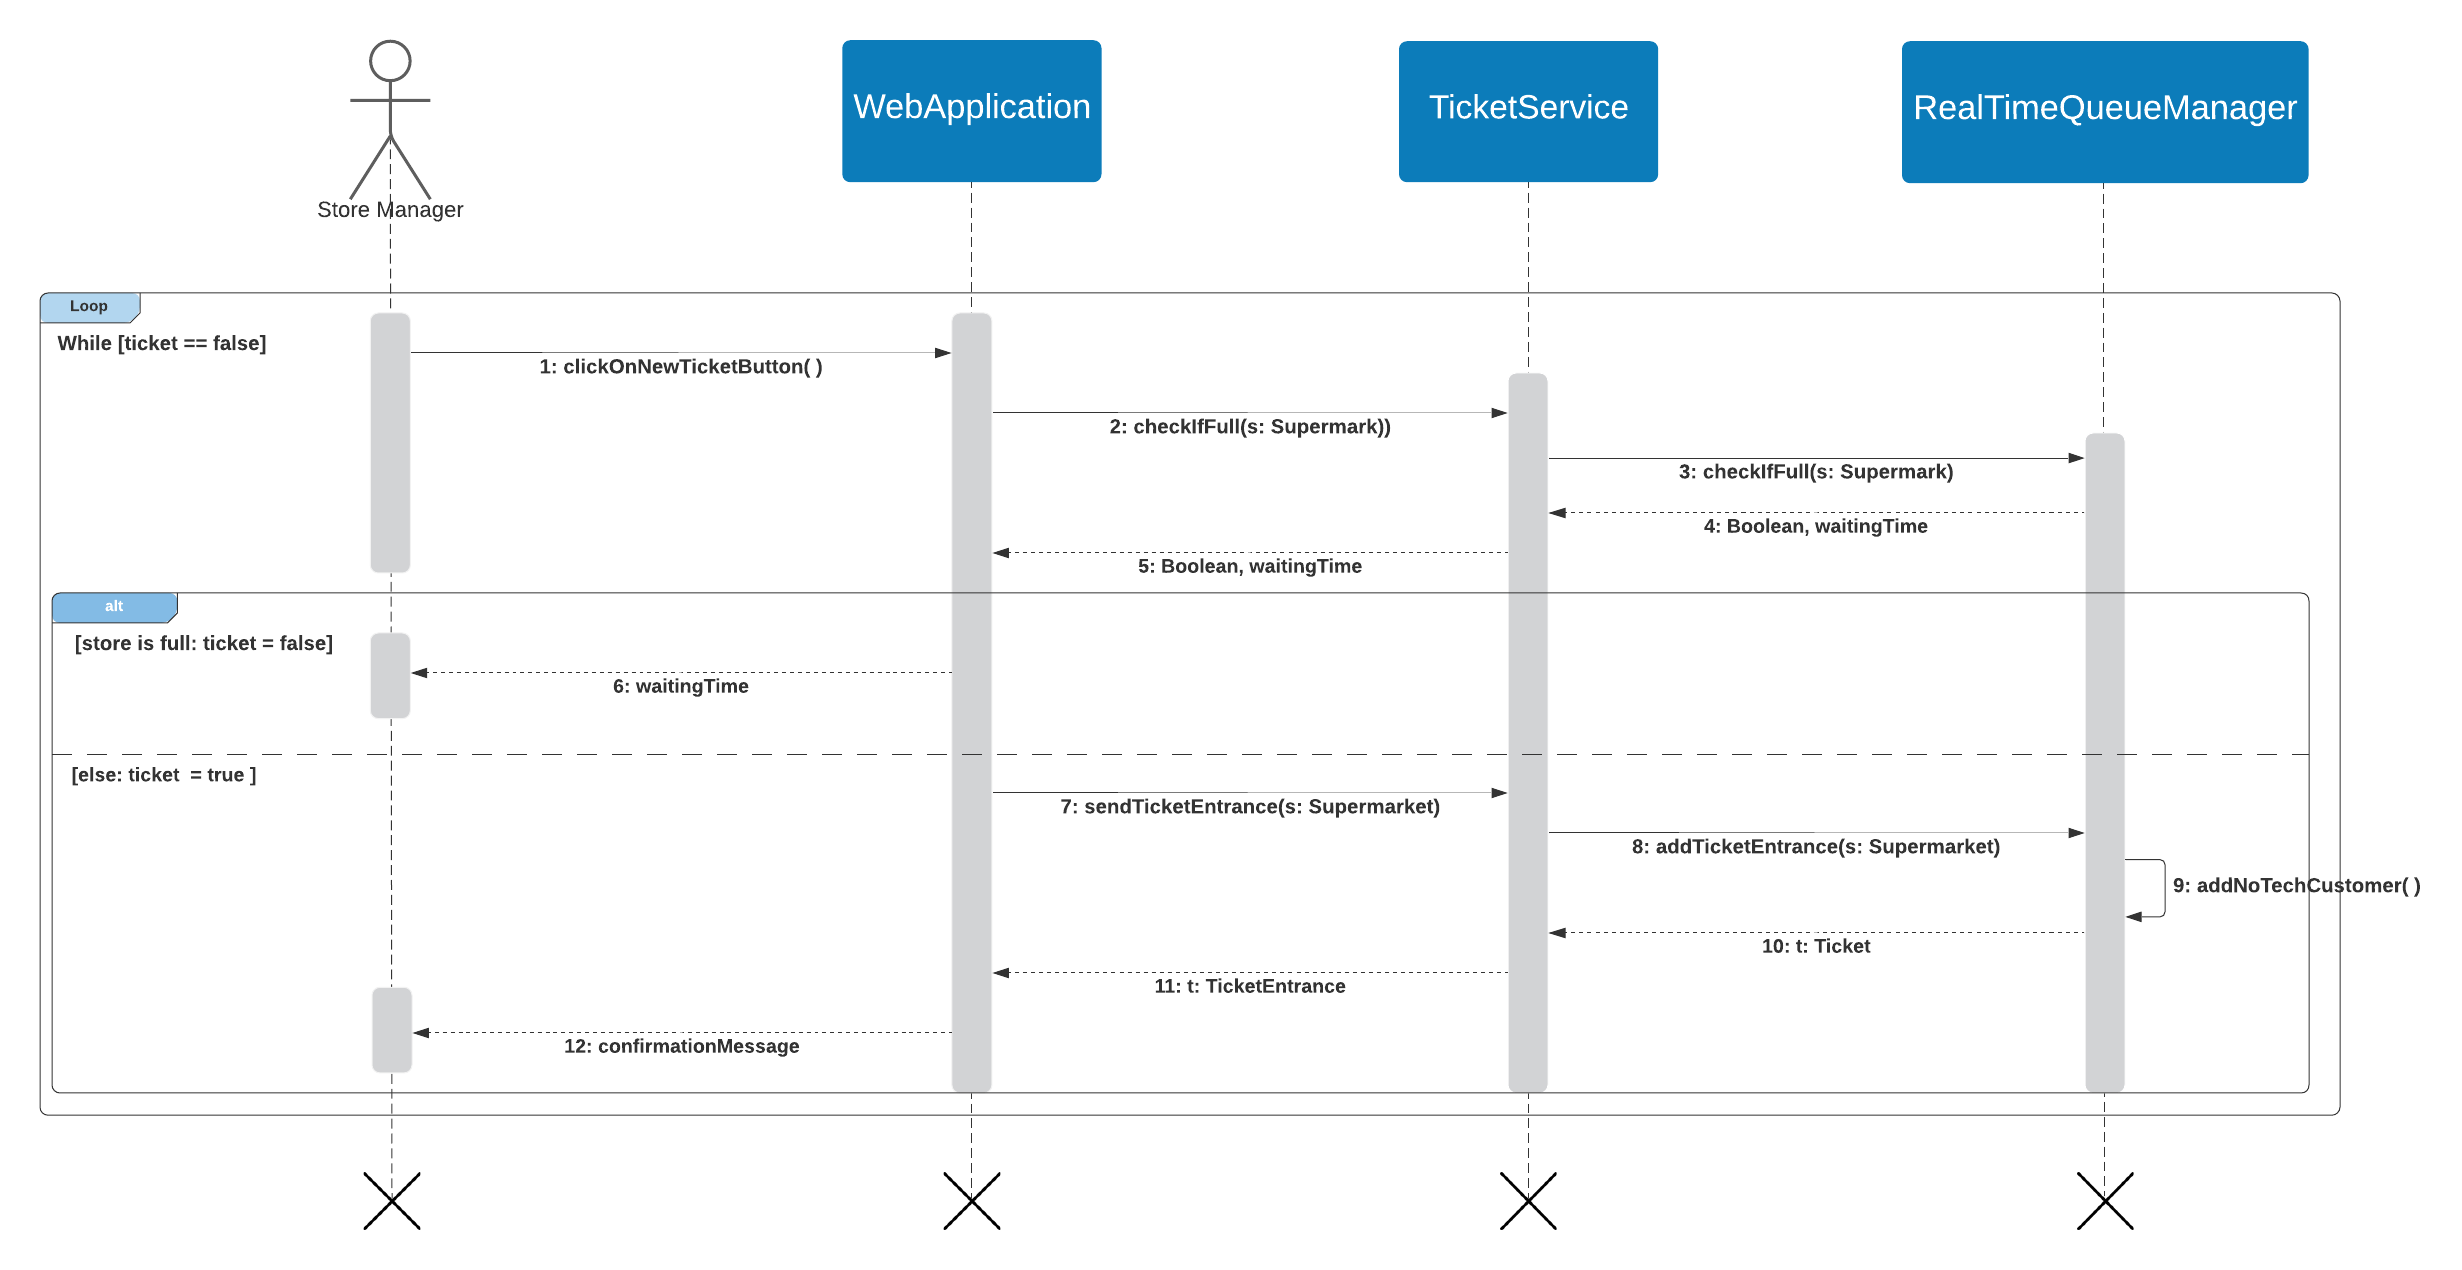
\includegraphics[scale=0.5]{./TicketGenerationSequenceDD}}
\caption{Ticket Generation Sequence Diagram}
\end{figure}


\subsection{Send Notification}
This sequence diagram shows the mechanism through which the Customer is notified. \\
In particular, the MobileApplication exploits the GPSService to retrieve the position from the GoogleMapsService. A second similar request is done to retrieve the tripTime: at this point the MobileApplication check the WaitingTime and the tripTime values and when these two are equal, sends a notification to the Customer.
\begin{figure}[H]
\centerline{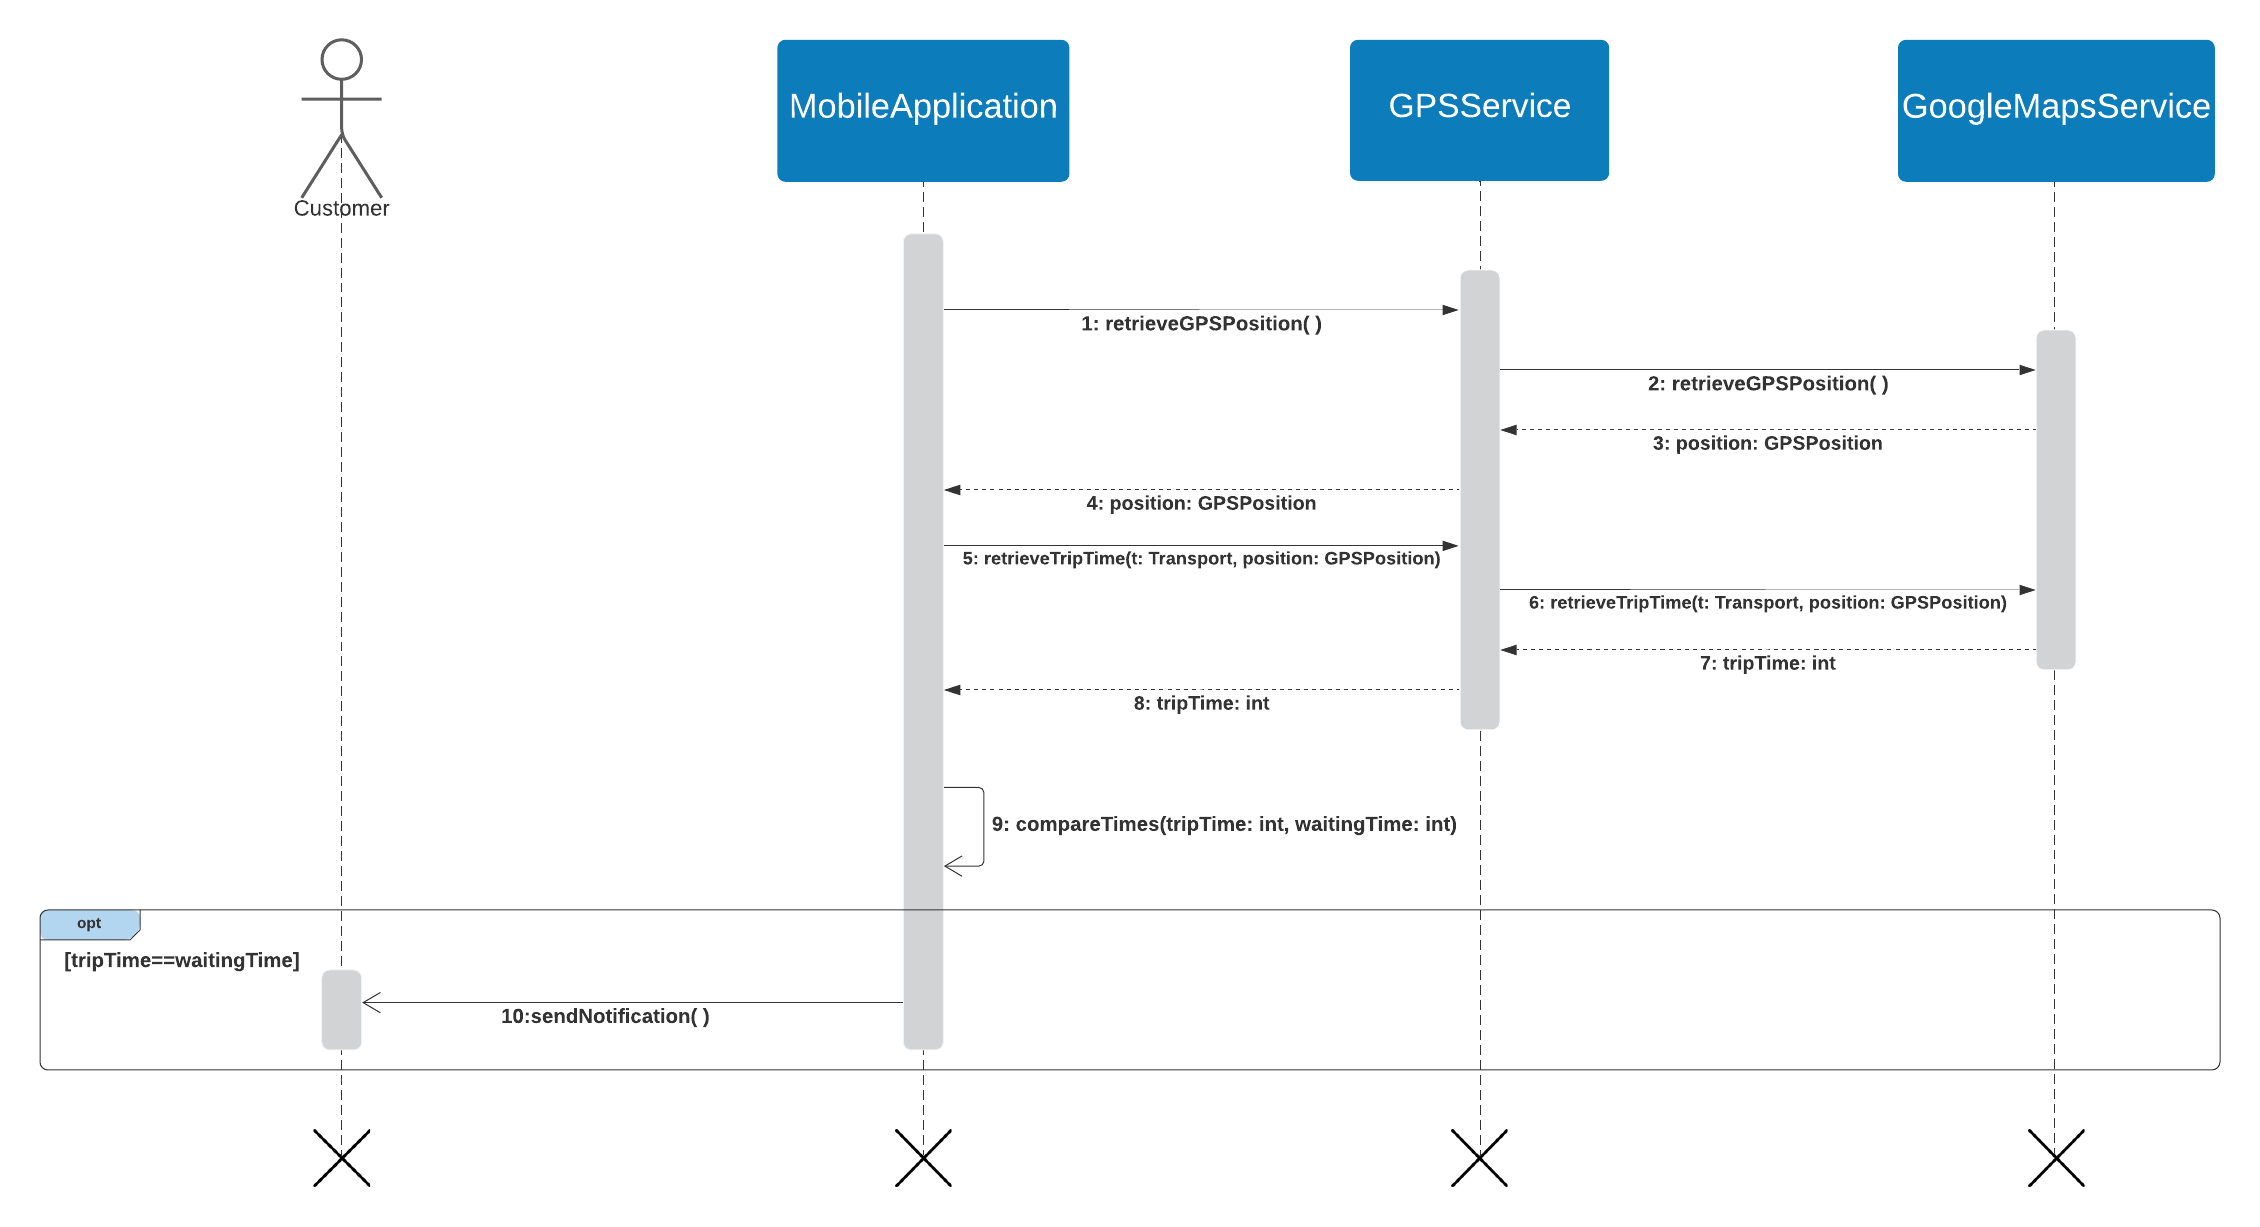
\includegraphics[scale=0.5]{./SendNotificationSequenceDD}}
\caption{Send Notification Sequence Diagram}
\end{figure}



\subsection{Check Affluence}
In this diagram is shown how a Store Manager can check the affluence if his supermarket. After he has logged in in the and has clicked on the Affluence tab, the WebApplication calls the AffluenceService. This last component calls the RealTimeQueueManager and can return all the needed informations.
\begin{figure}[H]
\centerline{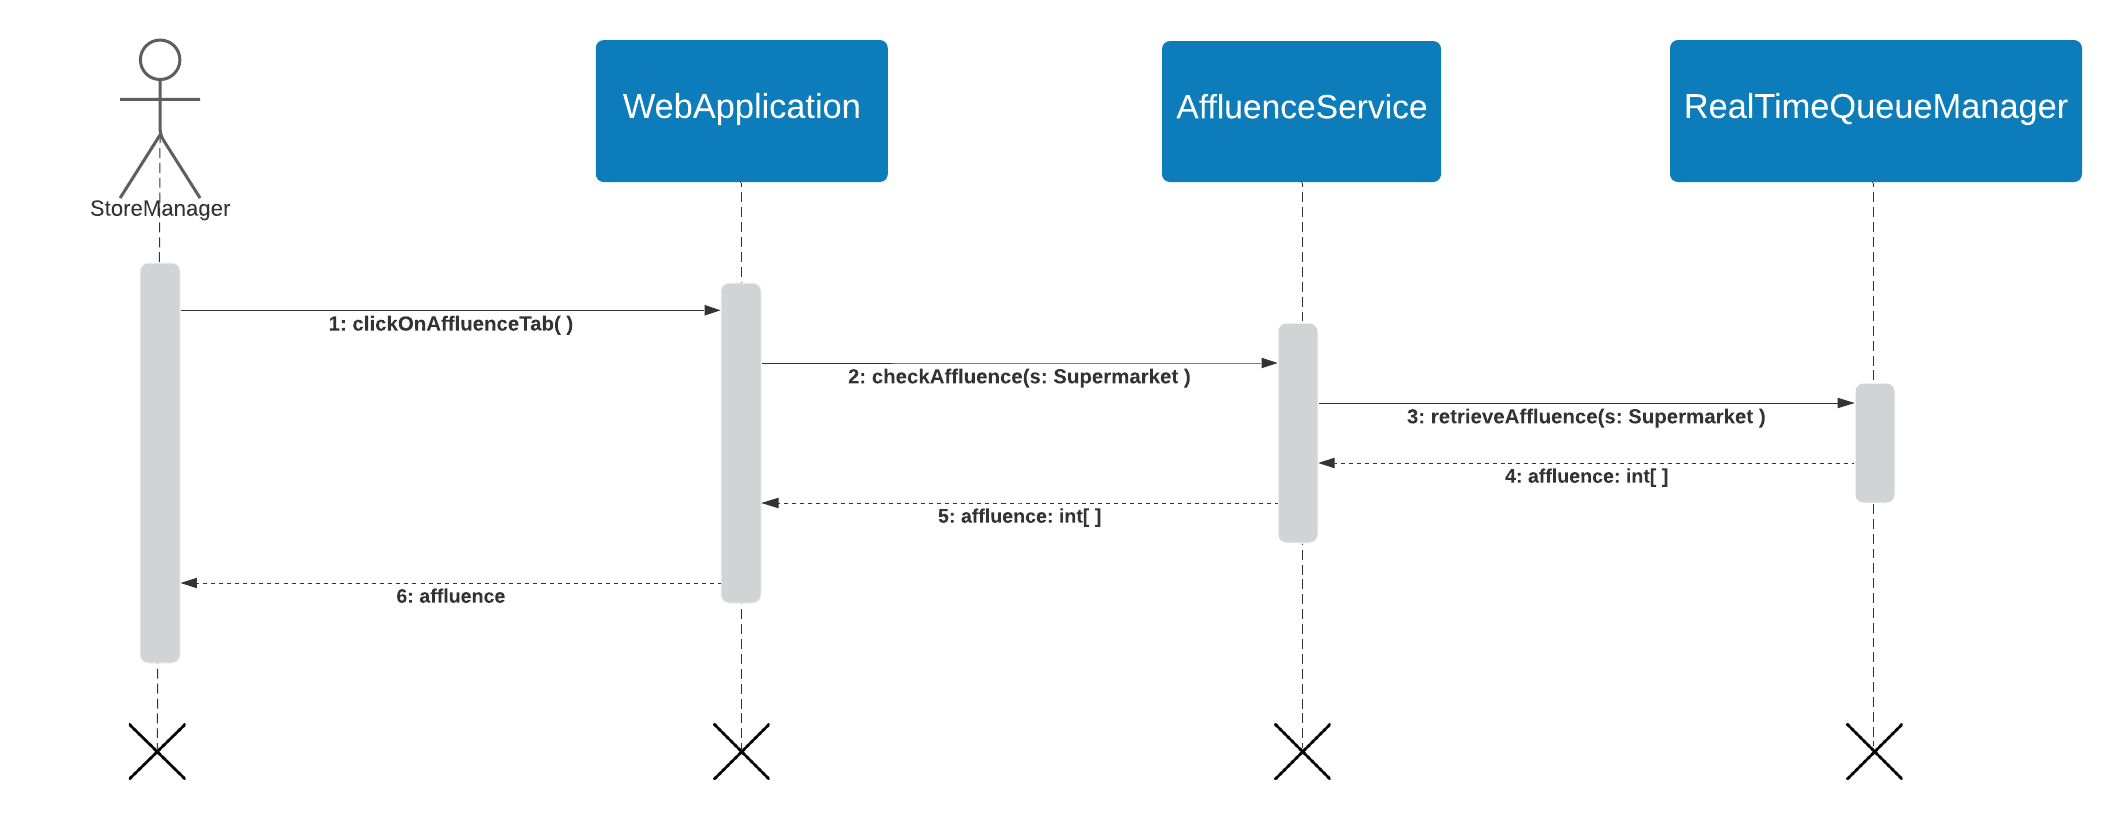
\includegraphics[scale=0.5]{./CheckAffluenceSequenceDD}}
\caption{Check Affluence Sequence Diagram}
\end{figure}



\subsection{Check Bookings}
In this diagram is shown how a Store Manager can check the bookings if his supermarket. After he has logged in in the and has clicked on the Booking tab, the WebApplication calls the AffluenceService. This last component calls the DatabaseAccess component that can retrieve all the needed informations from the Database.
\begin{figure}[H]
\centerline{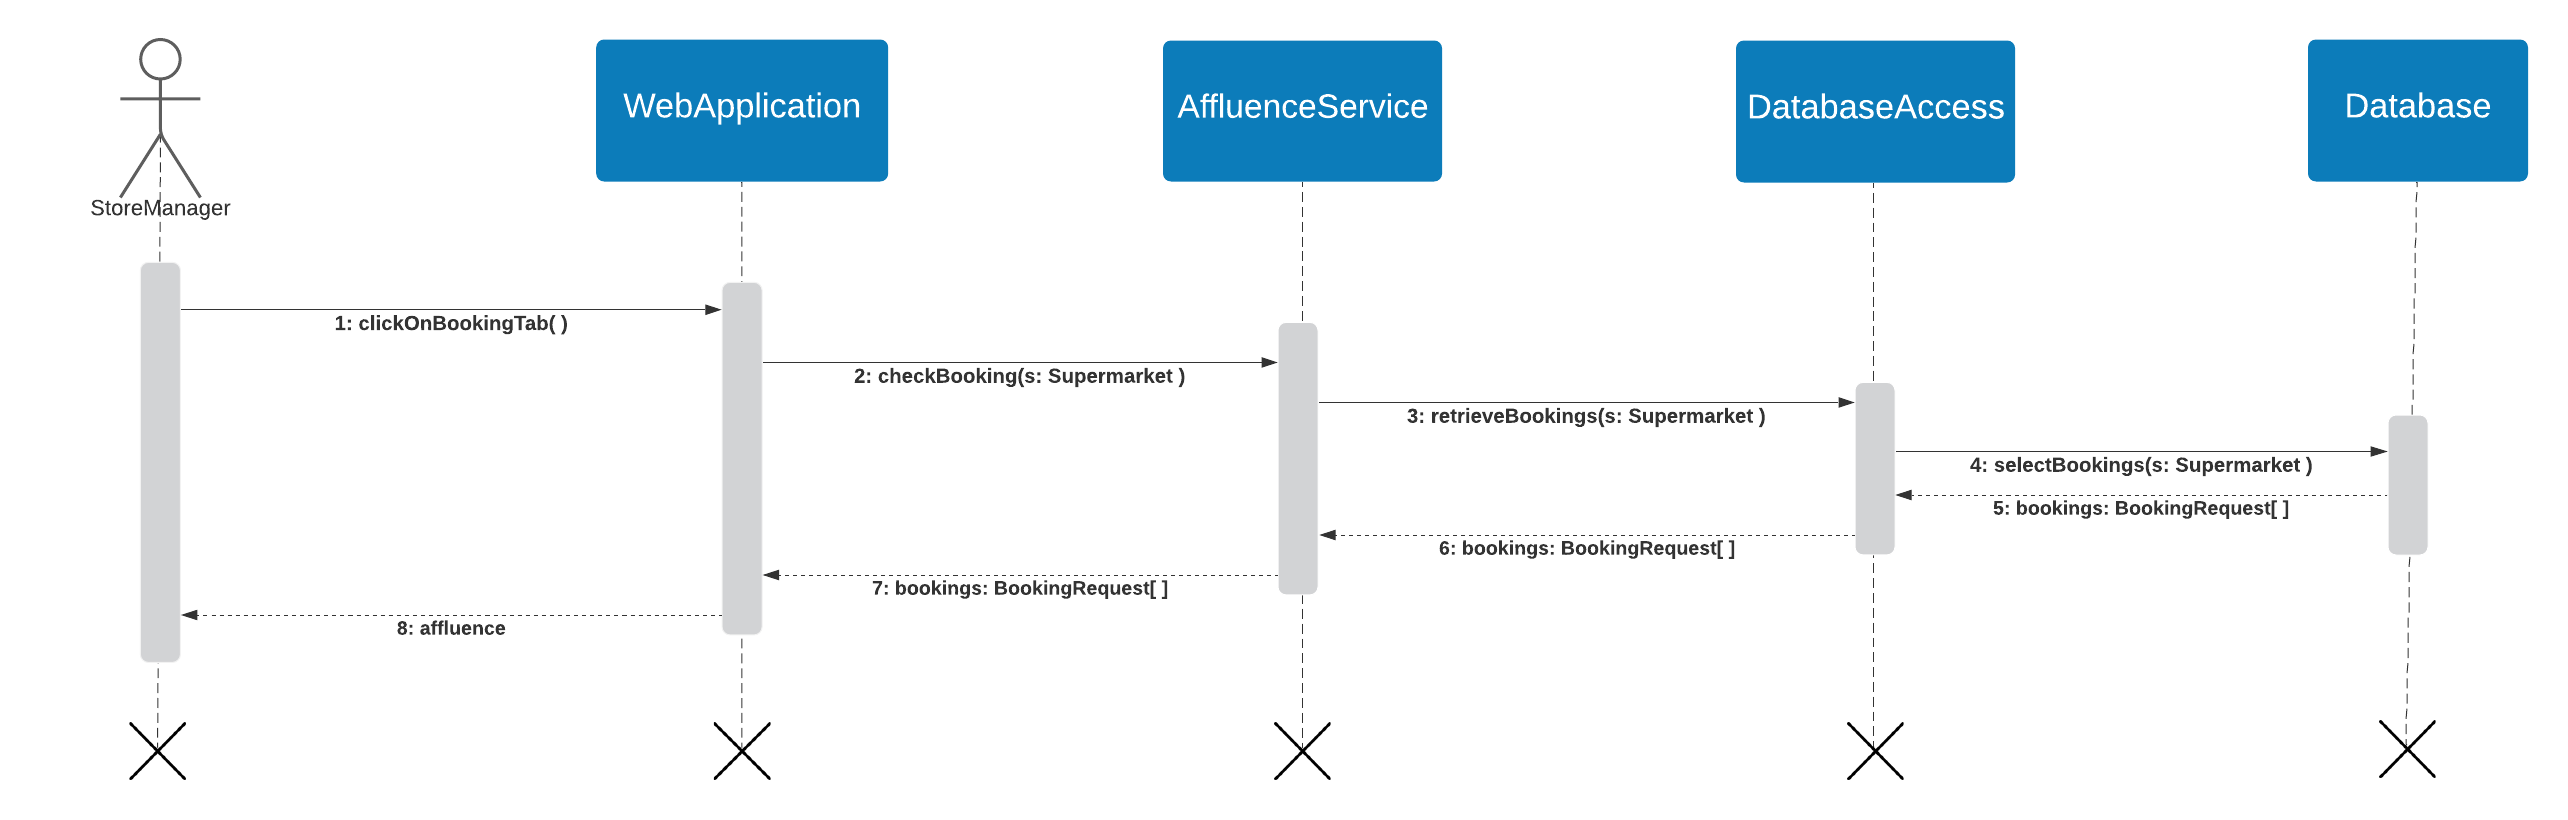
\includegraphics[scale=0.5]{./CheckBookingsSequenceDD}}
\caption{Check Bookings Sequence Diagram}
\end{figure}


 
 